% !TeX root = ../main.tex
% Add the above to ea  ch chapter to make compiling the PDF easier in some editors.

\chapter{Flow Models}\label{section:flow_models}

\section{Overview}

We train our flow using \textit{flow matching} \citep{lipmanFlowMatchingGenerative2023,albergoStochasticInterpolantsUnifying2023,liuFlowStraightFast2022}, which generalizes diffusion models with a more flexible design space. In this section we first formulate the flow matching objective (Sec. \ref{section:flow_matching}), explain the design choices it enables (Sec. \ref{section:design_choices}), and describe in more detail how samples (Sec. \ref{section:sampling_integration}) and likelihoods (Sec. \ref{section:computing_likelihoods}) can be obtained using a flow model. 

\section{Flow Matching} \label{section:flow_matching}

Flow matching, first proposed in \citep{lipmanFlowMatchingGenerative2023,albergoStochasticInterpolantsUnifying2023,liuFlowStraightFast2022} (see \citep{lipmanFlowMatchingGuide2024} for a recent comprehensive overview), aims to solve the problem of \textit{dynamic transport}, i.e. finding a time-dependent vector field to transport the source (prior) distribution $p_0$ to the target (data) distribution $p_1$. More formally, the vector field $u_t: [0,1] \times \R^d \to \R^d$ leads to the ordinary differential equation (ODE)
\begin{equation} \label{eq:ode}
    dx = u_t(x) dt
\end{equation}
and induces a \textit{flow} $\phi: [0,1] \times \R^d \to \R^d$ that gives the solution to the ODE at time $t$ with starting point $x_0$, such that 
\begin{align}
    \frac{d}{dt} \phi_t(x_0) &= u_t(\phi_t(x_0)) \\
    \phi_0(x_0) &= x_0.
\end{align}
Starting with $p_0$, transformed distributions $p_t$ can then be defined using this flow with the push-forward operation
\begin{equation}
    p_t := [\phi_t]_\# (p_0)
\end{equation} 
and the instantaneous change in the density satisfies the \textit{continuity equation}
\begin{equation}
    \frac{\partial p}{\partial t} = - \nabla \cdot (p_t u_t)
\end{equation}
which means that probability mass is conserved during the transformation. With these formulations, we say the vector field $u_t$ \textit{generates} the \textit{probability path} (also called \textit{interpolant}) $p_t$.

\subsection{The Objective}

The formulation above could also be applied to traditional continuous normalizing flows (CNFs) \citep{chenNeuralOrdinaryDifferential2018a}, and flow matching is an instantiation of CNFs. However, continuous normalizing flows have in the past been trained using objectives which required solving and then backpropagating through the ODE, such as KL-divergence or other likelihood-based objectives, which made training costly. This problem was later addressed with diffusion models and their simpler regression objectives such as score matching and denoising \citep{sohl-dicksteinDeepUnsupervisedLearning2015, songScoreBasedGenerativeModeling2021a,hoDenoisingDiffusionProbabilistic2020} that proved to be very effective. The flow matching objective is also formulated as a simulation-free regression objective, and is more flexible than the diffusion objectives. 

As explained in Section \ref{section:flow_matching}, the goal in flow matching is to learn a vector field $v_\theta: [0,1] \times \R^d \to \R^d$ parametrized by a neural network.\footnote{For conciseness, we interchangeably use the subscripts for vector fields to denote time ($u_t(x)$) and parameters ($v_\theta(t,x)$).} If we know the ground truth vector field $u$ and can sample from the intermediate $p_t$'s, we can directly optimize the flow matching objective 
\begin{equation} \label{eq:fm_objective}
    \Lfm := \bbE_{t \sim \U(0,1), x_t \sim p_t(x)} \Vert v_\theta(t, x_t) - u_t(x_t) \Vert ^2
\end{equation}
by first sampling a time point $t$ and then $x_t \sim p_t$. However in practice, we neither have a closed form expression for $u$ nor can sample from an arbitrary $p_t$ without integrating the flow. 

The \textit{conditional flow matching} (CFM) framework first introduced in \citep{lipmanFlowMatchingGenerative2023} and then extended in \citep{tongImprovingGeneralizingFlowbased2023} solves this problem by formulating the intermediate probability paths as mixtures of simpler paths, 
\begin{equation}
    p_t(x) = \int p_t(x \mid z) q(z) dz
\end{equation}
where $z$ is the conditioning variable and $q(z)$ a distribution over $z$ (e.g. with $z := (x_0, x_1), q(z) = p_0(x_0)p_1(x_1), u_t(x \mid z) = x_1 - x_0$, and $p_t(x \mid z) = \N(x \mid (1-t)x_0 + tx_1, \sigma^2)$). Then similar to how $p_t$'s were generated by the vector field $u_t$, the conditional probability paths $p_t(x \mid z)$ are generated by conditional vector fields $u_t(x \mid z)$, and as shown in \citep{tongImprovingGeneralizingFlowbased2023} $u_t$ can be decomposed in terms of these conditional vector fields as 
\begin{equation}
    u_t(x) = \bbE_{z \sim q(z)} \frac{u_t(x \mid z) p_t(x \mid z)}{p_t(x)}.
\end{equation}
Then similar to Equation \ref{eq:fm_objective}, we have the conditional flow matching objective 
\begin{equation} \label{eq:cfm_objective}
    \Lcfm := \bbE_{t \sim \U(0,1), z \sim q(z), x_t \sim p_t(x \mid z)}
    \Vert v_\theta(t, x_t) - u_t(x_t \mid z) \Vert ^2.
\end{equation}
That is, we first sample a conditioning variable $z$, and then regress to the \textit{conditional} vector field $u_t(x \mid z)$. Thus we obtain a tractable objective by defining sample-able conditional probability paths and a tractable conditional vector field. Moreover, as shown in \citep{tongImprovingGeneralizingFlowbased2023}, the FM and CFM objectives are equivalent up to a constant and therefore
\begin{equation}
    \nabla_\theta \Lfm = \nabla_\theta \Lcfm,
\end{equation}
meaning we do not lose the expressive power of the FM objective by regressing only to the conditional vector fields. As we will show in Section \ref{section:design_choices}, the choice of these conditional probability paths, vector fields, along with the conditioning variable itself, makes the flow matching approach particularly flexible.

\subsection{Training} \label{sec:fm_training}

To sum up the discussion in the previous section, a step of training a flow model using the CFM objective (Equation \ref{eq:cfm_objective}) proceeds as follows:
\begin{enumerate}
    \item Sample $t \sim \U(0,1), z \sim q(z)$, and $x_t \sim p_t(x \mid z)$.
    \item Compute $\Lcfm = \Vert v_\theta(t, x_t) - u_t(x_t \mid z) \Vert ^2$.
    \item Update $\theta$ with $\nabla_\theta \Lcfm$.
\end{enumerate}
An equivalent approach with the loss computed in the space our data lies is to predict the target $x_1$ rather than the velocity and compute the loss as $\Vert v_\theta(t,x_t) - x_1 \Vert^2$, and the velocity as $v_\theta(t, x_t) - x_0$ with $x_0$ the starting point for integration. 

\subsection{Couplings and Conditional Paths} \label{section:design_choices}

With this framework established, the three main design choices for building a flow matching model are choosing the coupling $q(z)$, the conditional ``ground truth'' vector field $u_t(x \mid z)$, and the conditional probability paths $p_t(x \mid z)$. Starting with an arbitrary source distribution $p_0$ and target distribution $p_1$, \citet{tongImprovingGeneralizingFlowbased2023} propose three different ways of constructing conditional paths from couplings between $p_0$ and $p_1$, of which we focus on two (independent and optimal transport couplings). In all setups, the condition variable $z$ corresponds to a pair $(x_0, x_1)$ of source and target points. 

\textbf{Independent Coupling.} The simplest way of obtaining is to sample independently from $p_0$ and $p_1$; i.e. $q(z) = p_0(x_0) p_1(x_1)$, with the conditional paths and the vector field defined as 
\begin{align} 
    p_t(x \mid z) &= \N(x \mid (1-t)x_0 + t x_1, \sigma^2) \label{eq:cond_path} \\
    u_t(x \mid z) &= x_1 - x_0. \label{eq:cond_vector_field}
\end{align}
The conditional paths and the coupling defined this was are easily easy to sample from, but have undesirable properties such as crossing paths which which can lead to high variance in the ground truth vector field for a specific point and time. Moreover in practice, independent couplings can lead to curved paths that incur higher integration errors, as there is no notion of straightness considered in this formulation.

\textbf{Optimal Transport.} To obtain straighter and shorter paths that are easier to integrate, \citet{tongImprovingGeneralizingFlowbased2023} propose to use the static 2-Wasserstein optimal transport map $\pi$ as the coupling; i.e.
\begin{equation}
    q(z) = \pi(x_0, x_1),
\end{equation}
with the conditional paths and vector field defined as in Equations \ref{eq:cond_path} and \ref{eq:cond_vector_field}. The flow model thus obtained solves the dynamic optimal OT problem as $\sigma^2 \to 0$ (Proposition 3.4 in \citep{tongImprovingGeneralizingFlowbased2023}). However, computing the exact OT map for the entire dataset is challenging, especially in high dimensions as in our problem. It can instead be approximated using mini-batches \citep{fatrasMinibatchOptimalTransport2021}. This means at the end the OT problem is solved only to an approximation, but nevertheless results in straighter paths that cross less often, since intuitively an $x_0 \sim p_0$ is more likely to be coupled with $x_1 \sim p_1$ closer to it rather than an $x_1$ chosen uniformly random.

\section{Riemannian Flow Matching} \label{sec:riemannian_fm}

When our data lies on a manifold, flow matching can be extended to define a flow over the manifold as well. Such an approach can both lead to a better scalable generative model by reducing the effective dimensionality of the problem, and make learning easier by introducing a strong inductive bias to the problem.  Discrete and continuous normalizing flows have previously been adapted to Riemannian manifolds \citep{gemiciNormalizingFlowsRiemannian2016,mathieuRiemannianContinuousNormalizing2020,louNeuralManifoldOrdinary2020}, and in this section we begin with a brief overview of Riemannian manifolds (we refer to textbooks on the topic such as \citep{johnm.leeIntroductionRiemannianManifolds2018} for a more rigorous treatment), and then explain how an ODE over a Riemannian manifold can be learned following the framework of Riemannian flow matching \citep{chenRiemannianFlowMatching2023}.\footnote{The presentation in this section is additionally based on the Geometric Generative Models tutorial by Joey Bose, Alexander Tong, and Heli Ben-Hamu at the 2024 Learning On Graphs Conference.} 

\subsection{A Brief Review of Riemannian Manifolds}

\begin{figure}[t!]
    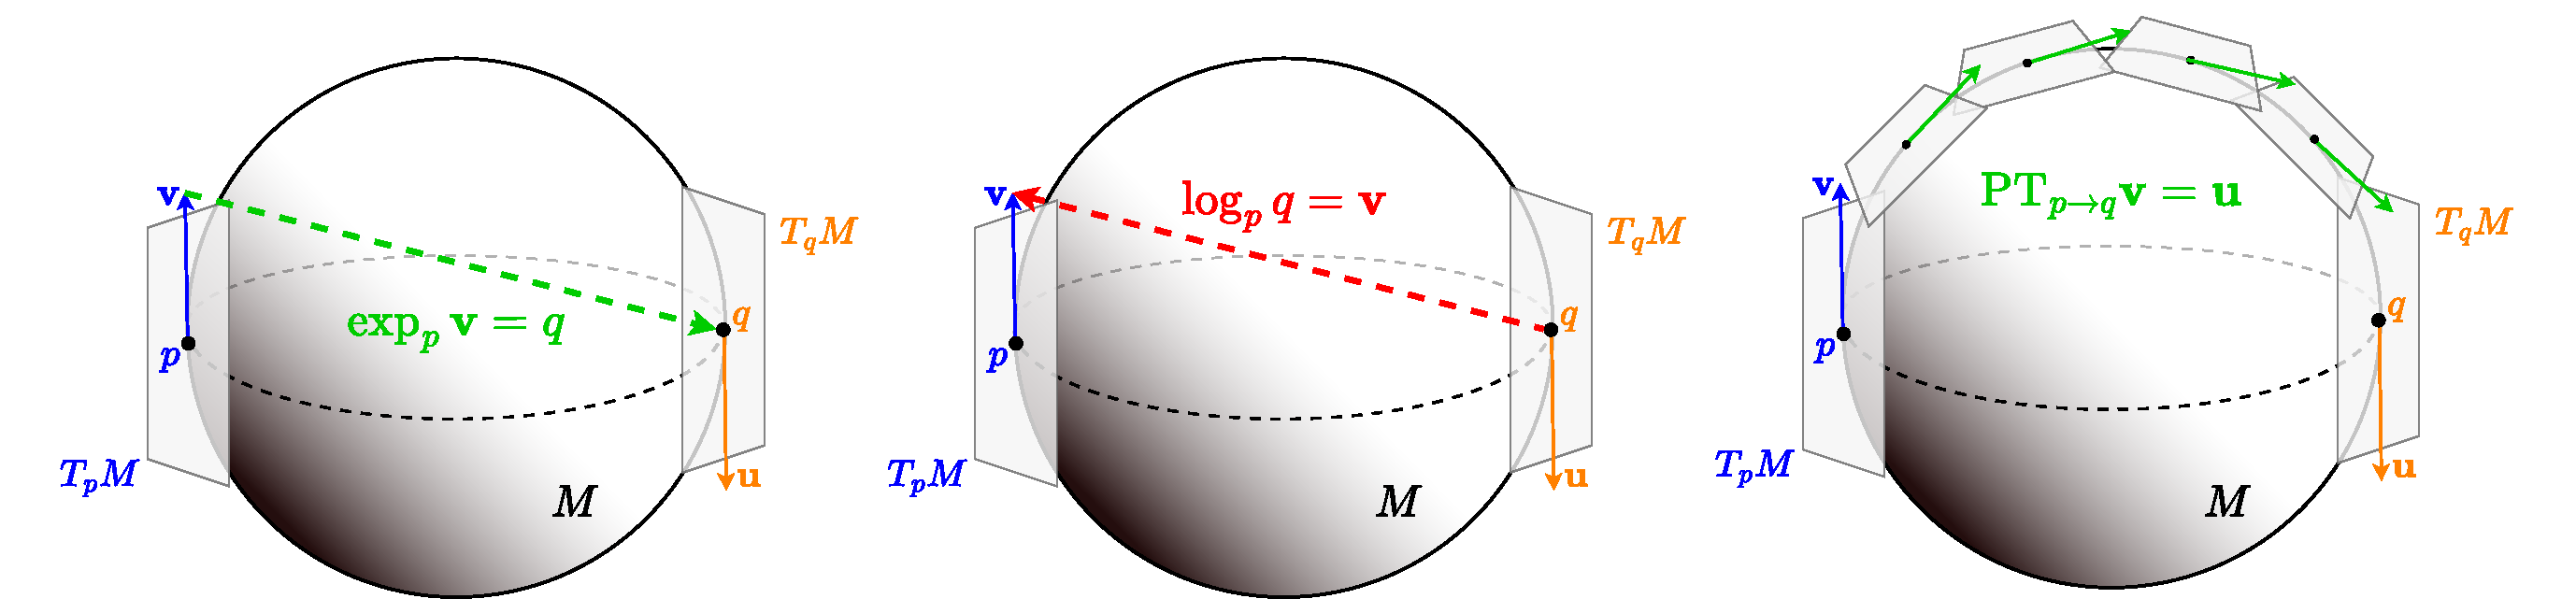
\includegraphics[width=\linewidth]{figures/manifolds.drawio.pdf}
    \caption{\label{fig:manifolds}\textbf{Visualizing the exponential, logarithmic, and parallel transport maps on a manifold.} The unique geodesic curve $\gamma$ between $p$ and $q$ with $\dot \gamma(0) = \mathbf{v}$ corresponds to the great circle of the sphere coinciding with the upper boundary in the diagrams.}    
\end{figure}

A smooth \textit{manifold} $M$ is a smooth topological space that is locally Euclidean. The local Euclidean structure is represented by \textit{charts} mapping open sets $U \subset M$ to $\R^n$. A set of charts covering the entire manifold is called an \textit{atlas}, and smoothness arises from the transitions between overlapping charts being smooth functions. Each point $x \in M$ is equipped with a tangent space $T_x M$ that is a vector space containing vectors tangent to $M$, such as velocities. In addition to being a smooth manifold, a Riemannian manifold also contains a Riemannian metric $g$ that defines an inner product $\langle u, v \rangle_g = u^T G v$ for $u, v \in T_x M$ and positive definite matrix $G$. A metric most importantly enables us to define angles and distances over the manifold as $\Vert u \Vert_g = \sqrt{\langle u, u\rangle_g} = \sqrt{u^T G u}$ and $\cos \theta = \frac{\langle u, v \rangle_g}{\Vert u \Vert_g \Vert v \Vert_g}$. 

A \textit{curve} is a smooth function $\gamma: [0, 1] \to M$, and tangent vectors $v \in T_x M$ can be expressed as time derivatives $\dot \gamma(t)$ of curves with $\gamma(t) = x$. Using the metric $g$, we can measure the length of a curve by computing the length of the tangent vector at each point along the curve:
\begin{equation}
    \vert \gamma \vert =
    \int_0^1 \Vert \dot \gamma (t) \Vert_g^2 dt.
\end{equation}
The ``shortest'' curve in this sense connecting two points $x,y\in M$ is called a \textit{geodesic}. We can thus define a distance between two points as the length of a (not necessarily unique) geodesic connecting them. 

A manifold is also equipped with three operations that we will make use of: the \textit{exponential map}, the \textit{logarithmic} map, and \textit{parallel transport} (see Figure \ref{fig:manifolds} for a visual depiction). The exponential map $\exp_x: T_x M \to M$ at a point $x \in M$ maps a tangent vector $v$ to the point $\gamma(1) \in M$ where $\gamma$ is the unique geodesic satisfying $\gamma(0) = x$ and $\dot \gamma(0) = v$. The logarithmic map $\log_x: M \to T_x M$ maps a point $y \in M$ back to the tangent vector $v := \dot \gamma (0)$. It is generally the inverse of the exponential map. Finally the parallel transport map $\text{PT}_{x \to y}: T_x M \to T_y M$ transports a tangent vector $v := \dot \gamma(0)$ along the geodesic with $\gamma(1) = y$ keeping the lengths and angles between the transported vectors constant. Together, these three operations allow us to move along geodesics with tangent vectors as the velocities, and transport tangent vectors to the same tangent space to be able to compute distances between them, which are all steps required to build a flow model over a Riemannian manifold. 

\subsection{Flow Models over Manifolds}

Riemannian flow matching (RFM) \citep{chenRiemannianFlowMatching2023} extends the flow matching framework to Riemannian manifolds. As the three key design choices, we need to define a coupling $q$, conditional probability paths $p_t$, and a conditional vector field $u_t$. 

A coupling can be defined simply by sampling $x_0 \sim p_0$ and $x_1 \sim p_1$ independently, or with a mini-batch optimal transport map with the distances defined above using geodesics. For $t\in [0,1]$, the geodesic interpolation $x_t \sim p_t(x_t \mid x_0, x_1)$ (analogous to linear interpolation in Euclidean space) between $x_0$ and $x_1$ is computed as 
\begin{equation}
    x_t := \exp_{x_0}(t \log_{x_0} x_1)
\end{equation}
and the conditional vector field $u_t$ as
\begin{equation}
    u_t(x_t \mid x_0, x_1) := \frac{\log_{x_t}x_1}{1 - t}.
\end{equation}
Finally to solve the ODE, we compute one Euler integration step as
\begin{align}
    dx_t &= u_t(x_t)dt \\
    x_{t + 1} &= \exp_{x_t}(v_\theta(t, x_t) \Delta t)
\end{align}
where $\Delta t$ is the step size. 


\section{Computing Likelihoods} \label{section:computing_likelihoods}

In earlier normalizing flows that aim to learn a static mapping between the two distributions \citep{rezendeVariationalInferenceNormalizing2015}, given source samples $x_0 \sim p_0$, likelihoods of the generated samples $z = f(x_0) \approx p_1$  can be computed exactly via the change of variables formula
\begin{equation} \label{eq:static_cov}
    \log p_1(z) = \log p_0(z) - \log \det \left\vert J_f(z) \right\vert
\end{equation}
where $J_f$ is the Jacobian of $f$. Thus, we can obtain exact likelihoods for the generated samples by taking the determinant of the Jacobian of the normalizing flow. Since Jacobian computations can be costly, this has motivated work on designing normalizing flows with easier to compute Jacobians, such as RealNVP \citep{dinhDensityEstimationUsing2017}. 

% Note that the terminology/notation etc are already set here
In a \textit{continuous normalizing flow} on the other hand, the \textit{instantaneous change of variables} formula \citep{chenNeuralOrdinaryDifferential2018a} defines the change in probability mass through time. Given that the vector field $v_t$ is continuous in $t$ and uniformly Lipschitz continuous in $\R^d$, it holds that
\begin{align} \label{eq:continuous_cov}
    \frac{d \log p_t(\phi_t(x))}{dt} &= - \divergence(v_t(\phi_t(x))) \\
                                     &= - \trace \left( \frac{d v_t(\phi_t(x))}{dt} \right)
\end{align}
where $\frac{d v_t(\phi_t(x))}{dt} =: J_v(\phi_t(x))$ is the Jacobian of the vector field. We integrate over time to compute the full change in probability:
\begin{equation} \label{eq:full_continuous_cov}
    \log p_1(\phi_1(x)) = \log p_0(\phi_0(x)) - \int_0^1 \trace(J_v(\phi_t(x))) dt.
\end{equation}
Then we can integrate the Jacobian trace of the vector field through time (simultaneously with sampling) to obtain exact likelihoods for the generated samples. 

\subsection{Faster Likelihoods Through Trace Estimation} \label{section:trace_estimation}

However, materializing the full Jacobian of the vector field can be prohibitively expensive, especially if the task is very high dimensional (as in our case) since the log determinant computation has a time complexity of $O(d^3)$ \citep{grathwohlFFJORDFreeformContinuous2018} without any restrictions on the structure of the Jacobian. 

To alleviate this problem, \citep{grathwohlFFJORDFreeformContinuous2018} propose to use the \textit{Hutchinson trace estimator} \citep{hutchinsonStochasticEstimatorTrace1990} for an unbiased estimate of the Jacobian trace of a square matrix: 
\begin{equation} \label{eq:hutchinson}
    \trace(J_v) = \bbE_{p(\epsilon)} \left[ \epsilon^T J_v \epsilon \right]
\end{equation}
where $p(\epsilon)$ is chosen such that $\bbE[\epsilon] = 0$ and $\Cov(\epsilon) = I$, typically a Gaussian or a Rademacher distribution. Then, we can use this estimator in place of the explicit trace computation in Equation \ref{eq:full_continuous_cov} and compute the likelihoods as
\begin{equation}
    \log p_1(\phi_1(x)) = \log p_0(\phi_0(x)) - \int_0^1 \bbE_{p(\epsilon)} \left[ \epsilon^T J_v(\phi_t(x)) \epsilon \right] dt.
\end{equation}

The performance benefit of using the Hutchinson trace estimator results from the fact that the Jacobian-vector product $J_v \epsilon$ can be computed very efficiently by automatic differentiation \citep{baydinAutomaticDifferentiationMachine2018}, giving the whole approach a time complexity of $O(d)$ only. Due to this significant performance improvement and being an unbiased estimate, the Hutchinson trace estimator has been widely used in the diffusion/flow model literature \citep{lipmanFlowMatchingGenerative2023,songScoreBasedGenerativeModeling2021a}.


